%This is a template file for use of iopjournal.cls

\documentclass{iopjournal}
\bibliographystyle{IEEEtran}
\usepackage{float}
\usepackage{amsmath}
\usepackage{tikz}
\usepackage{fix-cm} % Allow scalable Computer Modern fonts to avoid font substitution warnings

% Options
%  [anonymous]  Provides output without author names, affiliations or acknowledgments to facilitate double-anonymous peer-review
%
% The following packages are required by iopjournal.cls and do not need to be declared again:
%  graphicx
%  fancyhdr
%  xcolor
%  hyperref
%

\begin{document}

\articletype{Tarea 5} %	 e.g. Paper, Letter, Topical Review...

\title{Clasificador de Numeros Mnist}

\author{Daniel González$^1$\orcid{0000-0000-0000-0000}}

\affil{$^1$Facultad de Ingeniería, Universidad Autónoma de Querétaro, Querétaro, México \\ 09/10/2025}

\email{dgonzalez16@alumnos.uaq.mx}

\keywords{mnist, redes neuronales, perceptron, entrenamiento, clasificador, prediccion}

\begin{abstract}
Se desarrollo de un sistema sencillo de reconocimiento de numeros escritos a mano utilizando el 
conjunto de datos MNIST como base de entrenamiento además, se diseñó una interfaz gráfica en Python mediante la librería Tkinter, que 
permite al usuario dibujar un dígito en un lienzo digital y obtener 
de forma inmediata la clasificación realizada por el modelo entrenado. Se discutieron diferentes técnicas de preprocesamiento, 
como el escalado, centrado y normalización de la imagen a 28$\times$28 píxeles, con el objetivo de adaptar la entrada a las 
características del dataset MNIST.Los resultados muestran que la CNN alcanza una exactitud superior al 97\% en los datos de 
prueba y, es importante mencionar que la predicción de numeros escritos en la interfaz depende del estilo de escritura del usuario, 
la integración de un preprocesamiento adecuado mejora considerablemente la robustez del sistema. 
\end{abstract}

\section{Introducción}

El reconocimiento de patrones escritos a mano es uno de los problemas más comunes en el campo del aprendizaje automático, ya que representa 
un reto tanto por la variabilidad de la escritura humana es decir la caligrafia unica asi como por la necesidad de modelos eficientes. 
Uno de los conjuntos de datos más utilizados para abordar este problema es MNIST (Modified National Institute of Standards and Technology), 
el cual contiene 70,000 imágenes en escala de grises de dígitos manuscritos del 0 al 9, divididas en 60,000 para entrenamiento y 10,000 para 
prueba. 
\begin{figure}[H]
\centering
        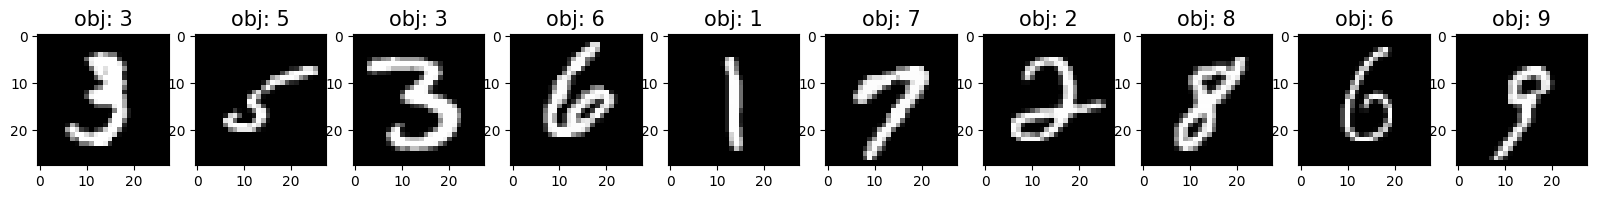
\includegraphics[width=0.7\textwidth]{../../img/mnist.png}
\caption{Ejemplos de numeros de la Mnist}\label{mnist}   
\end{figure}

Cada imagen tiene un tamaño de 28$\times$28 píxeles y constituye un estándar para la evaluación de algoritmos de clasificación de imágenes.

Entre los modelos más sencillos para abordar esta tarea se encuentra el perceptrón multicapa (MLP), una red neuronal artificial en la cual 
cada neurona de una capa se conecta con todas las de la siguiente. En este caso se implementó un perceptrón con una capa oculta y una capa 
de salida, entrenado sobre el dataset MNIST, para la tarea de clasificación de numeros. A pesar de ser una arquitectura simple, el 
perceptrón es capaz de aprender representaciones útiles que permiten un buen desempeño con este problema.

Para probar nuestro modelo, se diseñó además una interfaz gráfica en Python utilizando la librería \texttt{Tkinter}. 
Esta interfaz permite al usuario dibujar un numero en una ventana y recibir la predicción del modelo, integrando así el entrenamiento 
de la red neuronal con una aplicación interactiva. De igual manera, se exploraron técnicas de preprocesamiento de la imagen, como el escalado, 
centrado y normalización, con el objetivo de mejorar la correspondencia entre los dígitos dibujados por el usuario y aquellos 
contenidos en el dataset de entrenamiento.


\section{Desarrollo}
\subsection{Modelo}
Se implementó una red perceptron con entrada de 784 ya que al tener imagenes de 28$\times$28 sera nuestra entrada de datos `Aplanados', ademas
de esto se eligio como capa oculta 128 neuronas como numero promedio entre aprendizaje y tiempo de entrenamiento asi como una función de
activacion ReLU para que aprenda patrones no lineales. Por ultimo una salida de 10, que seran nuestros numeros del 0 al 9 con función de activacion
softmax para tener la probabilidad segun el modelo.
Se usó el optimizador Adam, muy eficiente y ampliamente utilizado en problemas de clasificación.
La función de pérdida \textit{Sparse Categorical Crossentropy} es la adecuada cuando las etiquetas (\texttt{y\_train}) son enteros (0--9) y no vectores one-hot. 
Por último, se eligieron 5 épocas para que un perceptrón aprenda MNIST sin sobreajustar demasiado. 
El \textit{batch size} de 128 representa un tamaño estándar que balancea memoria y velocidad, 
mientras que el parámetro \texttt{validation\_split} con valor de 0.1 indica que el 10\% de los datos de entrenamiento se reservan para validación, 
monitoreando el rendimiento en datos no vistos durante cada época.

\begin{figure}[H]
\centering
        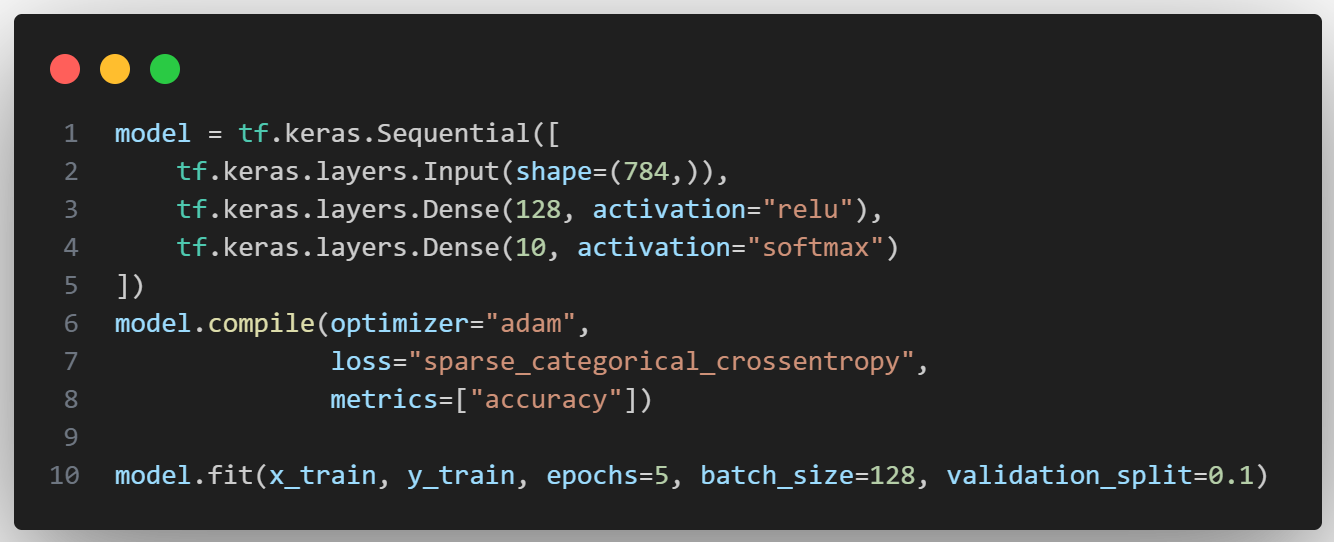
\includegraphics[width=0.7\textwidth]{rsc/modelo.png}
\caption{Parametros del Modelo Usado}\label{modelo}   
\end{figure}

Guardamos el modelo para no tener que entrenarlo cada vez que se corra el codigo y pasamos a la parte de diseñar nuestra interfaz.

\subsection{Interfaz}

Para el desarrollo de la interfaz gráfica en Python se uso la librería \texttt{Tkinter}. Esta interfaz tiene como objetivo permitir 
la interacción directa del usuario con el sistema de reconocimiento de numeros.

La aplicación presenta un lienzo digital de fondo negro sobre el cual el usuario puede dibujar un dígito mediante el cursor, 
utilizando un trazo blanco de grosor ajustable. Paralelamente, se emplea la librería \texttt{PIL} para almacenar el dibujo en una 
imagen procesable, lo que permite su posterior transformación al formato compatible con el modelo.

\begin{figure}[H]
\centering
        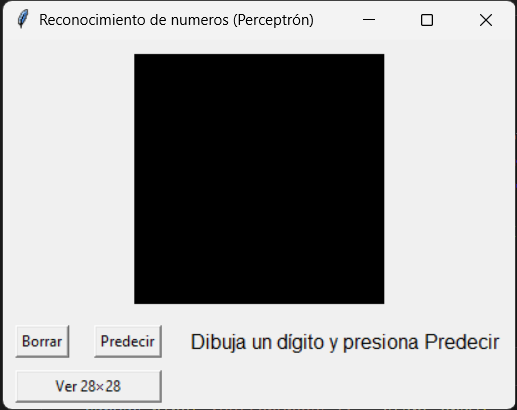
\includegraphics[width=0.5\textwidth]{rsc/Interfaz.png}
\caption{Interfaz Diseñada}\label{interfaz}   
\end{figure}

El preprocesamiento implementado consiste en escalar y centrar el dígito dentro de una imagen de 28$\times$28 píxeles, 
normalizar sus valores de intensidad y adaptarlo a la entrada esperada por el perceptrón. Una vez realizado este proceso, 
al presionar el botón \textit{Predecir}, la imagen es pasada al modelo previamente entrenado, mostrando en pantalla el resultado 
de la clasificación junto con la probabilidad asociada.

\begin{figure}[H]
\centering
        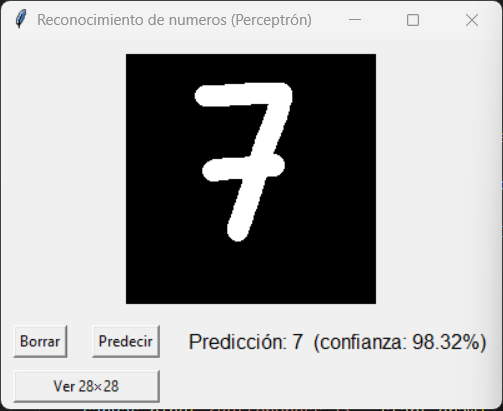
\includegraphics[width=0.5\textwidth]{rsc/Prediccion.png}
\caption{Predicción del Numero 7}\label{predicc}   
\end{figure}

La interfaz incluye también un botón \textit{Borrar}, que reinicia el lienzo para permitir múltiples intentos. De esta forma, 
se integran el entrenamiento del modelo y su uso práctico en tiempo real, proporcionando una herramienta sencilla e interactiva 
para la demostración del reconocimiento automático de dígitos escritos a mano.

Durante el desarrollo se enfrentaron problemas con este preprocesamiento ya que aunque nuestro modelo se entreno correctamente y nos 
mostraba buenos valores de accuracy la prediccion no era la mejor, debido a esto se implemento otro boton \textit{Ver28$\times$28} 
que nos permite ver la entrada que le llega a nuestro modelo, de esta manera nos aseguramos de ver lo mismo que el modelo en caso
de querer hacer un chequeo manual.

\begin{figure}[H]
\centering
        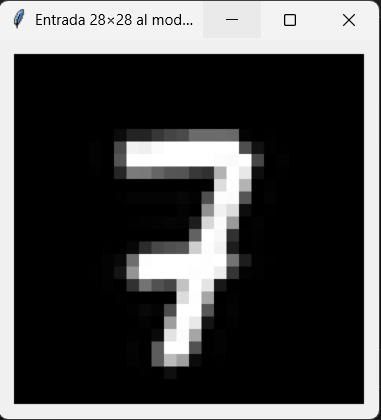
\includegraphics[width=0.5\textwidth]{rsc/entrada.png}
\caption{Entrada del modelo del numero 7 visto en la Figura~\ref{predicc}}\label{entrada}   
\end{figure}

\section{Conclusión}

El desarrollo de este proyecto permitió comprobar que un perceptrón multicapa, aun con una arquitectura sencilla, demuestra un desempeño 
notable para la de clasificación de dígitos manuscritos utilizando el conjunto de datos MNIST.\@
La integración con una interfaz gráfica demostró la utilidad práctica del modelo, ya que brindó la posibilidad de interactuar con el 
sistema asi como comprobar en tiempo real sus predicciones. Durante el proceso se demostro la importancia del preprocesamiento 
de las imágenes para lograr una correspondencia adecuada entre los datos de entrenamiento y los dígitos dibujados por el usuario, 
lo cual refleja un aspecto clave para mejorar la robustez del sistema.



%\begin{thebibliography}{00}
%\bibliography{references}
%\end{thebibliography}


\end{document}


